\subsection{Classifier-free Guidance and the Alignment-Fidelity Trade-off}

\begin{figure}
\centering
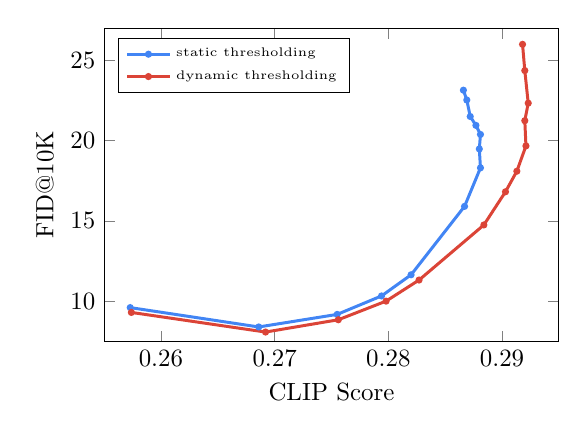
\begin{tikzpicture}[scale=0.9]

\definecolor{google_blue}{RGB}{66,133,244}
\definecolor{google_red}{RGB}{219,68,55}
\definecolor{google_yellow}{RGB}{194,144,0}
\definecolor{google_green}{RGB}{15,157,88}


\begin{axis}[
width=8cm,
height=6cm,
  xlabel=CLIP Score,
  ylabel=FID@10K,
  legend columns=1,
  legend pos=north west,
  legend style={font=\tiny},
  legend cell align=left,
  xmin=0.255,
  ymin=7.5,
  ymax=27,
  xmax=0.295,
  every axis plot/.append style={very thick}
]
\addplot +[mark=*, solid, google_blue, mark options={scale=0.4}] coordinates {(0.2573, 9.5976)(0.2686, 8.3913)(0.2755, 9.1741)(0.2794, 10.3238)(0.282, 11.6418)(0.2867, 15.9009)(0.2881, 18.2998)(0.288, 19.4781)(0.2881, 20.3822)(0.2877, 20.9476)(0.2872, 21.4995)(0.2869, 22.526)(0.2866, 23.1381)};

\addplot +[mark=*, solid, google_red, mark options={scale=0.4}] coordinates {(0.2574, 9.2972)(0.2692, 8.0746)(0.2756, 8.8401)(0.2798, 10.0002)(0.2827, 11.3142)(0.2884, 14.7455)(0.2903, 16.8102)(0.2913, 18.092)(0.2921, 19.6666)(0.292, 21.2374)(0.2923, 22.3307)(0.292, 24.3588)(0.2918, 25.9931)};


\legend{static thresholding, dynamic thresholding}
\end{axis}
\end{tikzpicture}
\caption{CLIP Score vs FID trade-off across various $\hat{\bx}_0$ thresholding methods for the 64$\times$64 model. We sweep over guidance values of $[1, 1.25, 1.5, 1.75, 2, 3, 4, 5, 6, 7, 8, 9, 10]$.
}
\label{fig:clip_vs_scaled_clip}
\end{figure}

\begin{figure}[tb]
\centering
\begin{subfigure}{.33\textwidth}
\centering
\setlength{\tabcolsep}{0.1pt}
\begin{tabular}{cccc}
\includegraphics[width=0.24\textwidth]{figures/clip_noclip_scaleclip/noclip/gw1_1.png.jpeg} &
\includegraphics[width=0.24\textwidth]{figures/clip_noclip_scaleclip/noclip/gw1_2.png.jpeg} &
\includegraphics[width=0.24\textwidth]{figures/clip_noclip_scaleclip/noclip/gw1_3.png.jpeg} &
\includegraphics[width=0.24\textwidth]{figures/clip_noclip_scaleclip/noclip/gw1_4.png.jpeg} \\ [-3pt]

\includegraphics[width=0.24\textwidth]{figures/clip_noclip_scaleclip/noclip/gw2_1.png.jpeg} &
\includegraphics[width=0.24\textwidth]{figures/clip_noclip_scaleclip/noclip/gw2_2.png.jpeg} &
\includegraphics[width=0.24\textwidth]{figures/clip_noclip_scaleclip/noclip/gw2_3.png.jpeg} &
\includegraphics[width=0.24\textwidth]{figures/clip_noclip_scaleclip/noclip/gw2_4.png.jpeg} \\ [-3pt]

\includegraphics[width=0.24\textwidth]{figures/clip_noclip_scaleclip/noclip/gw3_1.png.jpeg} &
\includegraphics[width=0.24\textwidth]{figures/clip_noclip_scaleclip/noclip/gw3_2.png.jpeg} &
\includegraphics[width=0.24\textwidth]{figures/clip_noclip_scaleclip/noclip/gw3_3.png.jpeg} &
\includegraphics[width=0.24\textwidth]{figures/clip_noclip_scaleclip/noclip/gw3_4.png.jpeg} \\ [-3pt]

\includegraphics[width=0.24\textwidth]{figures/clip_noclip_scaleclip/noclip/gw4_1.png.jpeg} &
\includegraphics[width=0.24\textwidth]{figures/clip_noclip_scaleclip/noclip/gw4_2.png.jpeg} &
\includegraphics[width=0.24\textwidth]{figures/clip_noclip_scaleclip/noclip/gw4_3.png.jpeg} &
\includegraphics[width=0.24\textwidth]{figures/clip_noclip_scaleclip/noclip/gw4_4.png.jpeg} \\ [-3pt]

\includegraphics[width=0.24\textwidth]{figures/clip_noclip_scaleclip/noclip/gw5_1.png.jpeg} &
\includegraphics[width=0.24\textwidth]{figures/clip_noclip_scaleclip/noclip/gw5_2.png.jpeg} &
\includegraphics[width=0.24\textwidth]{figures/clip_noclip_scaleclip/noclip/gw5_3.png.jpeg} &
\includegraphics[width=0.24\textwidth]{figures/clip_noclip_scaleclip/noclip/gw5_4.png.jpeg} \\
\end{tabular}
\vspace*{-0.2cm}
\caption{No thresholding.}
\end{subfigure}%
\hfill
\begin{subfigure}{.33\textwidth}
\centering
\setlength{\tabcolsep}{0.1pt}
\begin{tabular}{ccccc}
\includegraphics[width=0.24\textwidth]{figures/clip_noclip_scaleclip/clip/gw1_1.png.jpeg} &
\includegraphics[width=0.24\textwidth]{figures/clip_noclip_scaleclip/clip/gw1_2.png.jpeg} &
\includegraphics[width=0.24\textwidth]{figures/clip_noclip_scaleclip/clip/gw1_3.png.jpeg} &
\includegraphics[width=0.24\textwidth]{figures/clip_noclip_scaleclip/clip/gw1_4.png.jpeg} \\ [-3pt]

\includegraphics[width=0.24\textwidth]{figures/clip_noclip_scaleclip/clip/gw2_1.png.jpeg} &
\includegraphics[width=0.24\textwidth]{figures/clip_noclip_scaleclip/clip/gw2_2.png.jpeg} &
\includegraphics[width=0.24\textwidth]{figures/clip_noclip_scaleclip/clip/gw2_3.png.jpeg} &
\includegraphics[width=0.24\textwidth]{figures/clip_noclip_scaleclip/clip/gw2_4.png.jpeg} \\ [-3pt]

\includegraphics[width=0.24\textwidth]{figures/clip_noclip_scaleclip/clip/gw3_1.png.jpeg} &
\includegraphics[width=0.24\textwidth]{figures/clip_noclip_scaleclip/clip/gw3_2.png.jpeg} &
\includegraphics[width=0.24\textwidth]{figures/clip_noclip_scaleclip/clip/gw3_3.png.jpeg} &
\includegraphics[width=0.24\textwidth]{figures/clip_noclip_scaleclip/clip/gw3_4.png.jpeg} \\ [-3pt]

\includegraphics[width=0.24\textwidth]{figures/clip_noclip_scaleclip/clip/gw4_1.png.jpeg} &
\includegraphics[width=0.24\textwidth]{figures/clip_noclip_scaleclip/clip/gw4_3.png.jpeg} &
\includegraphics[width=0.24\textwidth]{figures/clip_noclip_scaleclip/clip/gw4_2.png.jpeg} &
\includegraphics[width=0.24\textwidth]{figures/clip_noclip_scaleclip/clip/gw4_4.png.jpeg} \\ [-3pt]

\includegraphics[width=0.24\textwidth]{figures/clip_noclip_scaleclip/clip/gw5_1.png.jpeg} &
\includegraphics[width=0.24\textwidth]{figures/clip_noclip_scaleclip/clip/gw5_2.png.jpeg} &
\includegraphics[width=0.24\textwidth]{figures/clip_noclip_scaleclip/clip/gw5_3.png.jpeg} &
\includegraphics[width=0.24\textwidth]{figures/clip_noclip_scaleclip/clip/gw5_4.png.jpeg} \\
\end{tabular}
\vspace*{-0.2cm}
\caption{Static thresholding.}
\end{subfigure}%
\hfill
\begin{subfigure}{.33\textwidth}
\centering
\setlength{\tabcolsep}{0.1pt}
\begin{tabular}{cccc}
\includegraphics[width=0.24\textwidth]{figures/clip_noclip_scaleclip/scaleclip/gw1_1.png.jpeg} &
\includegraphics[width=0.24\textwidth]{figures/clip_noclip_scaleclip/scaleclip/gw1_3.png.jpeg} &
\includegraphics[width=0.24\textwidth]{figures/clip_noclip_scaleclip/scaleclip/gw1_2.png.jpeg} &
\includegraphics[width=0.24\textwidth]{figures/clip_noclip_scaleclip/scaleclip/gw1_4.png.jpeg} \\ [-3pt]

\includegraphics[width=0.24\textwidth]{figures/clip_noclip_scaleclip/scaleclip/gw2_1.png.jpeg} &
\includegraphics[width=0.24\textwidth]{figures/clip_noclip_scaleclip/scaleclip/gw2_2.png.jpeg} &
\includegraphics[width=0.24\textwidth]{figures/clip_noclip_scaleclip/scaleclip/gw2_3.png.jpeg} &
\includegraphics[width=0.24\textwidth]{figures/clip_noclip_scaleclip/scaleclip/gw2_4.png.jpeg} \\ [-3pt]

\includegraphics[width=0.24\textwidth]{figures/clip_noclip_scaleclip/scaleclip/gw3_1.png.jpeg} &
\includegraphics[width=0.24\textwidth]{figures/clip_noclip_scaleclip/scaleclip/gw3_3.png.jpeg} &
\includegraphics[width=0.24\textwidth]{figures/clip_noclip_scaleclip/scaleclip/gw3_2.png.jpeg} &
\includegraphics[width=0.24\textwidth]{figures/clip_noclip_scaleclip/scaleclip/gw3_4.png.jpeg} \\ [-3pt]

\includegraphics[width=0.24\textwidth]{figures/clip_noclip_scaleclip/scaleclip/gw4_1.png.jpeg} &
\includegraphics[width=0.24\textwidth]{figures/clip_noclip_scaleclip/scaleclip/gw4_3.png.jpeg} &
\includegraphics[width=0.24\textwidth]{figures/clip_noclip_scaleclip/scaleclip/gw4_2.png.jpeg} &
\includegraphics[width=0.24\textwidth]{figures/clip_noclip_scaleclip/scaleclip/gw4_4.png.jpeg} \\ [-3pt]

\includegraphics[width=0.24\textwidth]{figures/clip_noclip_scaleclip/scaleclip/gw5_1.png.jpeg} &
\includegraphics[width=0.24\textwidth]{figures/clip_noclip_scaleclip/scaleclip/gw5_3.png.jpeg} &
\includegraphics[width=0.24\textwidth]{figures/clip_noclip_scaleclip/scaleclip/gw5_2.png.jpeg} &
\includegraphics[width=0.24\textwidth]{figures/clip_noclip_scaleclip/scaleclip/gw5_4.png.jpeg} \\
\end{tabular}
\vspace*{-0.2cm}
\caption{Dynamic thresholding.}
\end{subfigure}

\caption{Thresholding techniques on $256\times256$ samples for ``A photo of an astronaut riding a horse.'' Guidance weights increase from 1 to 5 as we go from top to bottom. No thresholding results in poor images with high guidance weights. Static thresholding is an improvement but still leads to oversaturated samples. Our dynamic thresholding leads to the highest quality images.  See \cref{fig:clip_vs_scaled_clip_samples} for more  qualitative comparison.}
\label{fig:clip_noclip_scaledclip}
\end{figure}

\begin{figure}[tb]
\centering
\begin{subfigure}{.495\textwidth}
\centering
\setlength{\tabcolsep}{0.1pt}
\begin{tabular}{cccc}
\includegraphics[width=0.24\textwidth]{figures/clip_vs_scaled_clip/clip_samples/1.jpg} &
\includegraphics[width=0.24\textwidth]{figures/clip_vs_scaled_clip/clip_samples/2.jpg} &
\includegraphics[width=0.24\textwidth]{figures/clip_vs_scaled_clip/clip_samples/3.jpg} &
\includegraphics[width=0.24\textwidth]{figures/clip_vs_scaled_clip/clip_samples/4.jpg} \\ [-3pt]

\includegraphics[width=0.24\textwidth]{figures/clip_vs_scaled_clip/clip_samples/5.jpg} &
\includegraphics[width=0.24\textwidth]{figures/clip_vs_scaled_clip/clip_samples/6.jpg} &
\includegraphics[width=0.24\textwidth]{figures/clip_vs_scaled_clip/clip_samples/7.jpg} &
\includegraphics[width=0.24\textwidth]{figures/clip_vs_scaled_clip/clip_samples/8.jpg} \\ [-3pt]

\includegraphics[width=0.24\textwidth]{figures/clip_vs_scaled_clip/clip_samples/9.jpg} &
\includegraphics[width=0.24\textwidth]{figures/clip_vs_scaled_clip/clip_samples/10.jpg} &
\includegraphics[width=0.24\textwidth]{figures/clip_vs_scaled_clip/clip_samples/11.jpg} &
\includegraphics[width=0.24\textwidth]{figures/clip_vs_scaled_clip/clip_samples/12.jpg} \\ [-3pt]

\includegraphics[width=0.24\textwidth]{figures/clip_vs_scaled_clip/clip_samples/13.jpg} &
\includegraphics[width=0.24\textwidth]{figures/clip_vs_scaled_clip/clip_samples/14.jpg} &
\includegraphics[width=0.24\textwidth]{figures/clip_vs_scaled_clip/clip_samples/15.jpg} &
\includegraphics[width=0.24\textwidth]{figures/clip_vs_scaled_clip/clip_samples/16.jpg} \\
\end{tabular}
\vspace*{-0.2cm}
\caption{Samples using static thresholding.}
\end{subfigure}%
\begin{subfigure}{.495\textwidth}
\centering
\setlength{\tabcolsep}{0.1pt}
\begin{tabular}{cccc}
\includegraphics[width=0.24\textwidth]{figures/clip_vs_scaled_clip/scaled_clip_samples/1.jpg} &
\includegraphics[width=0.24\textwidth]{figures/clip_vs_scaled_clip/scaled_clip_samples/2.jpg} &
\includegraphics[width=0.24\textwidth]{figures/clip_vs_scaled_clip/scaled_clip_samples/3.jpg} &
\includegraphics[width=0.24\textwidth]{figures/clip_vs_scaled_clip/scaled_clip_samples/4.jpg} \\[-3pt] 

\includegraphics[width=0.24\textwidth]{figures/clip_vs_scaled_clip/scaled_clip_samples/5.jpg} &
\includegraphics[width=0.24\textwidth]{figures/clip_vs_scaled_clip/scaled_clip_samples/6.jpg} &
\includegraphics[width=0.24\textwidth]{figures/clip_vs_scaled_clip/scaled_clip_samples/7.jpg} &
\includegraphics[width=0.24\textwidth]{figures/clip_vs_scaled_clip/scaled_clip_samples/8.jpg} \\[-3pt]

\includegraphics[width=0.24\textwidth]{figures/clip_vs_scaled_clip/scaled_clip_samples/9.jpg} &
\includegraphics[width=0.24\textwidth]{figures/clip_vs_scaled_clip/scaled_clip_samples/10.jpg} &
\includegraphics[width=0.24\textwidth]{figures/clip_vs_scaled_clip/scaled_clip_samples/11.jpg} &
\includegraphics[width=0.24\textwidth]{figures/clip_vs_scaled_clip/scaled_clip_samples/12.jpg} \\[-3pt]

\includegraphics[width=0.24\textwidth]{figures/clip_vs_scaled_clip/scaled_clip_samples/13.jpg} &
\includegraphics[width=0.24\textwidth]{figures/clip_vs_scaled_clip/scaled_clip_samples/14.jpg} &
\includegraphics[width=0.24\textwidth]{figures/clip_vs_scaled_clip/scaled_clip_samples/15.jpg} &
\includegraphics[width=0.24\textwidth]{figures/clip_vs_scaled_clip/scaled_clip_samples/16.jpg} \\
\end{tabular}
\vspace*{-0.2cm}
\caption{Samples using dynamic thresholding ($p=99.5$)}
\end{subfigure}
\caption{Static vs.\ dynamic thresholding on non-cherry picked $256\times256$ samples using a guidance weight of 5 for both the base model and the super-resolution model, using the same random seed. The text prompt used for these samples is ``A photo of an astronaut riding a horse.'' When using high guidance weights, static thresholding often leads to oversaturated samples, while our dynamic thresholding yields more natural looking images.}
\label{fig:clip_vs_scaled_clip_samples}
\end{figure}


We observe that classifier-free guidance \cite{ho2021classifierfree} is a key contributor to generating samples with strong image-text alignment, this is also consistent with the observations of \cite{ramesh-dalle, ramesh-dalle2}. There is typically a trade-off between image fidelity and image-text alignment, as we iterate over the guidance weight. 
While previous work has typically used relatively small guidance weights, \name uses relatively large guidance weights for all three diffusion models.  We found this to yield a good balance of sample quality and alignment.
However, naive use of large guidance weights often produces relatively poor results. To enable the effective use of larger guidance we introduce several innovations, as described below.


\textbf{Thresholding Techniques}: First, we compare various thresholding methods used with classifier-free guidance. Fig.  \ref{fig:clip_vs_scaled_clip} compares the CLIP vs.\ FID-10K score pareto frontiers for various thresholding methods of the base text-to-image $64\times64$ model. We observe that our dynamic thresholding technique results in significantly better CLIP scores, and comparable or better FID scores than the static thresholding technique for a wide range of guidance weights. \cref{fig:clip_noclip_scaledclip} shows qualitative samples for thresholding techniques.

\textbf{Guidance for Super-Resolution}: We further analyze the impact of classifier-free guidance for our $64\times64 \rightarrow 256\times256$ model. \cref{fig:256x256_t_eval_and_gw} shows the pareto frontiers for CLIP vs. FID-10K score for the $64\times64 \rightarrow 256\times256$ super-resolution model. $\mathrm{aug\_level}$ specifies the level of noise augmentation applied to the input low-resolution image during inference ($\mathrm{aug\_level} = 0$ means no noise). We observe that $\mathrm{aug\_level} = 0$ gives the best FID score for all values of guidance weight. Furthermore, for all values of $\mathrm{aug\_level}$, we observe that FID improves considerably with increasing guidance weight upto around $7-10$. While generation using larger values of $\mathrm{aug\_level}$ gives slightly worse FID, it allows more varied range of CLIP scores, suggesting more diverse generations by the super-resolution model. In practice, for our best samples, we generally use $\mathrm{aug\_level}$ in $[0.1, 0.3]$. Using large values of $\mathrm{aug\_level}$ and high guidance weights for the super-resolution models, \name can create different variations of a given $64\times64$ image by altering the prompts to the super-resolution models (See \cref{fig:super_res_variations} for examples).

\textbf{Impact of Conditioning Augmentation}: \cref{fig:super_res_ablation} shows the impact of training super-resolution models with noise conditioning augmentation. Training with no noise augmentation generally results in worse CLIP and FID scores, suggesting noise conditioning augmentation is critical to attaining best sample quality similar to prior work \cite{ho2021cascaded}. Interestingly, the model trained without noise augmentation has much less variations in CLIP and FID scores across different guidance weights compared to the model trained with conditioning augmentation. We hypothesize that this is primarily because strong noise augmented training reduces the low-resolution image conditioning signal considerably, encouraging higher degree of dependence on conditioned text for the model. 

\begin{figure}[t]
    \centering
    \begin{subfigure}[t]{0.49\textwidth}
    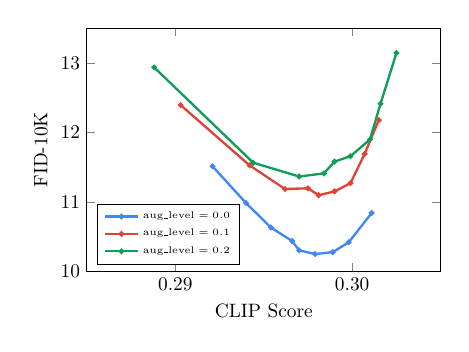
\begin{tikzpicture}[scale=0.7]

\definecolor{google_blue}{RGB}{66,133,244}
\definecolor{google_red}{RGB}{219,68,55}
\definecolor{google_yellow}{RGB}{194,144,0}
\definecolor{google_green}{RGB}{15,157,88}


\begin{axis}[width=8cm, height=6cm,
  xlabel=CLIP Score,
  ylabel=FID-10K,
  legend columns=1,
  legend pos=south west,
  legend style={font=\tiny},
  xmin=0.285,
  ymin=10.0,
  ymax=13.5,
  xmax=0.305,
  xtick = {0.29, 0.30},
  xticklabels = {0.29, 0.30},
  every axis plot/.append style={very thick}
]
\addplot +[mark=*, solid, google_blue, mark options={scale=0.4}] coordinates {(0.2921, 11.5138)(0.294, 10.9842)(0.2954, 10.6339)(0.2966, 10.4398)(0.297, 10.3053)(0.2979, 10.2523)(0.2989, 10.2793)(0.2998, 10.4203)(0.3011, 10.8419)};

\addplot +[mark=*, solid, google_red, mark options={scale=0.4}] coordinates {(0.2903, 12.3925)(0.2942, 11.526)(0.2962, 11.1867)(0.2975, 11.1969)(0.2981, 11.0975)(0.299, 11.1523)(0.2999, 11.2705)(0.3007, 11.6897)(0.3015, 12.176)};

\addplot +[mark=*, solid, google_green, mark options={scale=0.4}] coordinates {(0.2888, 12.9354)(0.2944, 11.5655)(0.297, 11.3662)(0.2984, 11.4112)(0.299, 11.5807)(0.2999, 11.658)(0.301, 11.8975)(0.3016, 12.4118)(0.3025, 13.143)};

\legend{$\mathrm{aug\_level} = 0.0$, $\mathrm{aug\_level} = 0.1$, $\mathrm{aug\_level} = 0.2$}
\end{axis}
\end{tikzpicture}
    \caption{Comparison between different values of $\mathrm{aug\_level}$.}
     \label{fig:256x256_t_eval_and_gw}
    \end{subfigure}
    \begin{subfigure}[t]{0.49\textwidth}
     \centering
     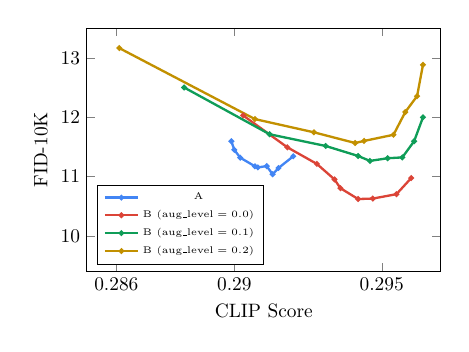
\begin{tikzpicture}[scale=0.7]

\definecolor{google_blue}{RGB}{66,133,244}
\definecolor{google_red}{RGB}{219,68,55}
\definecolor{google_yellow}{RGB}{194,144,0}
\definecolor{google_green}{RGB}{15,157,88}


\begin{axis}[width=8cm, height=6cm,
  xlabel=CLIP Score,
  ylabel=FID-10K,
  legend columns=1,
  legend pos=south west,
  legend style={font=\tiny},
  xmin=0.285,
  ymin=9.4,
  ymax=13.5,
  xmax=0.297,
  xtick = {0.286, 0.29, 0.295},
  xticklabels = {0.286, 0.29, 0.295},
  every axis plot/.append style={very thick}
]
\addplot +[mark=*, solid, google_blue, mark options={scale=0.4}] coordinates {(0.2899, 11.5946)(0.29, 11.45)(0.2902, 11.3181)(0.2907, 11.1728)(0.2908, 11.1542)(0.2911, 11.1761)(0.2913, 11.038)(0.2915, 11.1443)(0.292, 11.341)};
\addplot +[mark=*, solid, google_red, mark options={scale=0.4}] coordinates {(0.2903, 12.029)(0.2918, 11.4921)(0.2928, 11.2132)(0.2934, 10.9514)(0.2936, 10.8039)(0.2942, 10.6215)(0.2947, 10.6294)(0.2955, 10.7032)(0.296, 10.974)};
\addplot +[mark=*, solid, google_green, mark options={scale=0.4}] coordinates {(0.2883, 12.4993)(0.2912, 11.7119)(0.2931, 11.5148)(0.2942, 11.3467)(0.2946, 11.2633)(0.2952, 11.3083)(0.2957, 11.3226)(0.2961, 11.5953)(0.2964, 11.9972)};
\addplot +[mark=*, solid, google_yellow, mark options={scale=0.4}] coordinates {(0.2861, 13.1623)(0.2907, 11.9674)(0.2927, 11.745)(0.2941, 11.5647)(0.2944, 11.5996)(0.2954, 11.7032)(0.2958, 12.0862)(0.2962, 12.3539)(0.2964, 12.8817)};
\legend{ A,  B ($\mathrm{aug\_level} = 0.0$),  B ($\mathrm{aug\_level} = 0.1$),  B ($\mathrm{aug\_level} = 0.2$)}
\end{axis}
\end{tikzpicture}
      \caption{Comparison between training with no noise augmentation ``A'' vs noise augmentation ``B''}
      \label{fig:super_res_ablation}
    \end{subfigure}
    \caption{CLIP vs FID-10K pareto curves showing the impact of noise augmentation on our $64\times64 \rightarrow 256\times256$ model. For each study, we sweep over guidance values of $[1, 3, 5, 7, 8, 10, 12, 15, 18]$}
\end{figure}

\begin{figure}[t]
\captionsetup[subfigure]{labelformat=empty}
\centering
\begin{tabular}{c|@{\hskip 6pt}c@{\hskip 2pt}c@{\hskip 2pt}c}
Input & Unmodified & Oil Painting & Illustration \\
\begin{subfigure}[t]{0.24\textwidth} \centering \includegraphics[width=\textwidth]{figures/super_res_variations/64x64_2.jpeg} \caption{} \end{subfigure} &
\begin{subfigure}[t]{0.24\textwidth} \centering \includegraphics[width=\textwidth]{figures/super_res_variations/original2.jpeg} \caption{} \end{subfigure} &
\begin{subfigure}[t]{0.24\textwidth} \centering \includegraphics[width=\textwidth]{figures/super_res_variations/oil_painting2.jpeg} \caption{} \end{subfigure} &
\begin{subfigure}[t]{0.24\textwidth} \centering \includegraphics[width=\textwidth]{figures/super_res_variations/illustration2.jpeg} \caption{} \end{subfigure} \\[-12pt]

\begin{subfigure}[t]{0.24\textwidth} \centering \includegraphics[width=\textwidth]{figures/super_res_variations/64x64_3.jpeg} \caption{} \end{subfigure} &
\begin{subfigure}[t]{0.24\textwidth} \centering \includegraphics[width=\textwidth]{figures/super_res_variations/original3.jpeg} \caption{} \end{subfigure} &
\begin{subfigure}[t]{0.24\textwidth} \centering \includegraphics[width=\textwidth]{figures/super_res_variations/oil_painting3.jpeg} \caption{} \end{subfigure} &
\begin{subfigure}[t]{0.24\textwidth} \centering \includegraphics[width=\textwidth]{figures/super_res_variations/illustration3.jpeg} \caption{} \end{subfigure} \\[-12pt]

\begin{subfigure}[t]{0.24\textwidth} \centering \includegraphics[width=\textwidth]{figures/super_res_variations/64x64_4.jpeg} \caption{} \end{subfigure} &
\begin{subfigure}[t]{0.24\textwidth} \centering \includegraphics[width=\textwidth]{figures/super_res_variations/original4.jpeg} \caption{} \end{subfigure} &
\begin{subfigure}[t]{0.24\textwidth} \centering \includegraphics[width=\textwidth]{figures/super_res_variations/oil_painting4.jpeg} \caption{} \end{subfigure} &
\begin{subfigure}[t]{0.24\textwidth} \centering \includegraphics[width=\textwidth]{figures/super_res_variations/illustration4.jpeg} \caption{} \end{subfigure} \\

\end{tabular}
\caption{Super-resolution variations for some $64\times64$ generated images. We first generate the 64$\times$64 image using ``A photo of ... .''. Given generated $64\times64$ images, we condition both the super-resolution models on different prompts in order to generate different upsampled variations. e.g. for oil painting we condition the super-resolution models on the prompt ``An oil painting of ... .''. Through a combination of large guidance weights and $\mathrm{aug\_level} = 0.3$ for both super-res models we can generate different styles based on the style query through text.}
\label{fig:super_res_variations}
\end{figure}